\documentclass[12pt]{article}
%\setlength{\oddsidemargin}{0in}
%\setlength{\topmargin}{0.0in}
%\setlength{\textwidth}{6.7in}
%\setlength{\textheight}{8.5in}
%
\usepackage{graphicx}
\usepackage{enumitem}
\usepackage{mathtools}
\usepackage[usenames,dvipsnames]{xcolor}

\usepackage{geometry}
 \geometry{
 letterpaper,
 textwidth=6.5in
 }
\usepackage[utf8]{inputenc}
%\usepackage{libertine}
%\usepackage{libertinust1math}
\usepackage[libertine,cmintegrals,cmbraces,vvarbb]{newtxmath}
%\usepackage{newtxmath}
%\usepackage[osf]{ebgaramond}
\usepackage[T1]{fontenc}
%\usepackage{palatino}
\usepackage{microtype}

\usepackage{fancyhdr}
%\usepackage[colorlinks=true]{hyperref}

\pagestyle{fancy}
\fancyhf{}
\fancyhead[RE,LO]{\textcolor{BlueViolet}{Vibrations and Waves}}
\fancyhead[LE,RO]{ph2a: 2017}
\fancyfoot[RE,LO]{\textcolor{Orange}{Caltech}}
\fancyfoot[LE,RO]{\textcolor{Orange}{Physics, Math, and Astronomy}}

%\input mydefs.tex
\def\vev#1{\left\langle #1\right\rangle}
\def\hb{\hfill\break}
%
\begin{document}
%
\begin{centering}
\LARGE{QP 7: Newton's Rings}
\end{centering}
\bigskip
\bigskip

A plano-convex lens, which is cut from a spherical piece of glass with
radius $R$, rests on a flat glass plate as shown in Fig.~1. Light of
wavelength $\lambda$ is incident normally from above and is reflected at the
air\,--\,glass interfaces. The reflected beams then interfere to produce a
series of alternately bright and dark concentric circles when viewed
from above called Newton’s rings. A typical example is shown in Fig.~2. 
In this problem we will derive a quantitative understanding of
Newton’s rings.

\begin{figure}[!h]
  \centering
  \begin{minipage}[b]{0.45\textwidth}
    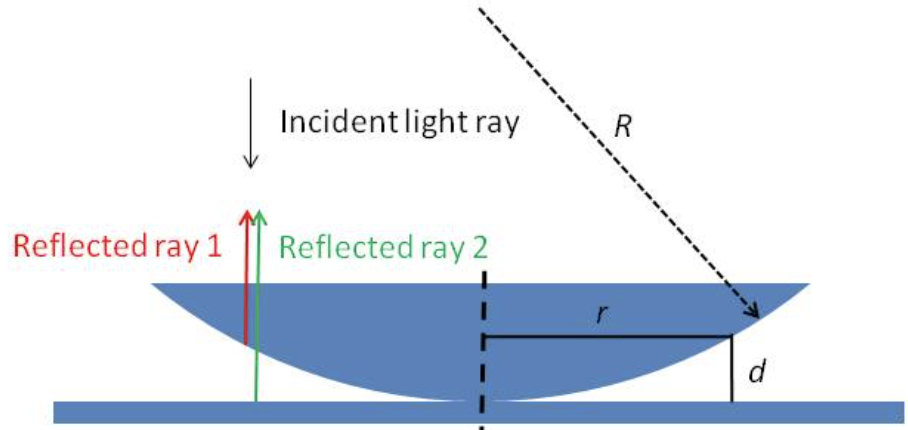
\includegraphics[width=\textwidth]{Lens.png}
    \caption{}
  \end{minipage}
  \begin{minipage}[b]{0.45\textwidth}
    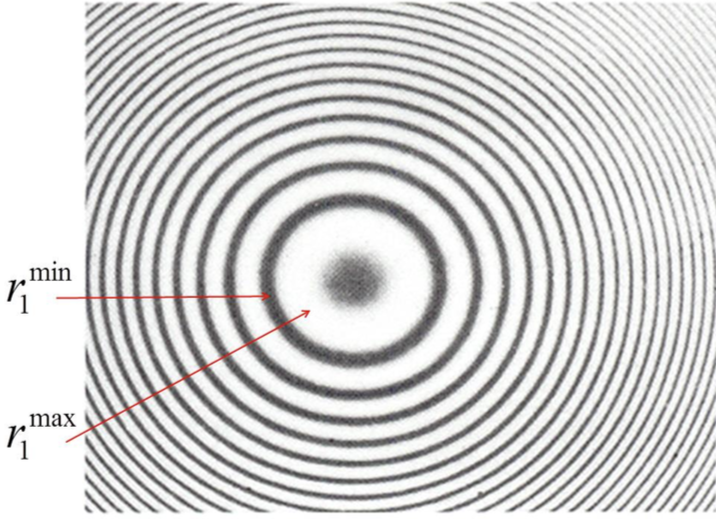
\includegraphics[width=\textwidth]{Rings.png}
    \caption{}
  \end{minipage}
\end{figure}

\begin{enumerate}[label=(\alph*)]
\item (5 pts)
Find an expression for the radial distance $r$ at which the separation between the spherical surface and the flat plate upon which it rests is $d$ as shown in Fig.~1. Make the approximation that $d << R$. 

\item (5 pts)
Consider reflection only from the two interfaces shown in Fig.~1,
which are denoted by reflected rays 1 \& 2. Assuming negligible bending
of the light rays, what is the phase difference between reflected rays
1 \& 2? Note that light undergoes a $\pi$ phase shift upon reflection at an
air\,--\,glass interface only when incident from the air side.

\item (5 point)
Derive an expression for the sets of radial distances $r_n^{max}$ and $r_n^{min}$
at which constructive and destructive interference of reflected rays 1
\& 2 occur respectively (see Fig.~2). Make use of your answer from
part (a).

\item (5 pts)
What is the difference in radii between the $n = 1$ and $n = 2$ dark rings
and what is the difference in radii between the $n = 25$ and $n = 26$ dark
rings assuming $R = 2$\,m and $\lambda = 640$\,nm? Comment on whether
this trend is consistent with Fig.~2.

\end{enumerate}
\bigskip


{\color{Sepia} \hrule}







\end{document}
